\section*{Appendix: Curve fitting}
In order to plot the evolution of both Lift and Drag for each phase, the computated velocity - solved from each respective ODE system - has been fitted from the resultant set of data points into a curve.\\
For this, the native \texttt{polyfit} and \texttt{poly2sym} \textsc{matlab} functions have ben employed. 

To correctly fit a set of points into a curve and avoid overfitting the polynomial (thus dealing with excessive oscillations and Runge's phenomemenon among others), the lienar Least Squares Method (LLS) has been used. The following plots show the square root sum and the norm of the squared regression value for each phase's velocity fit.

\begin{center}
	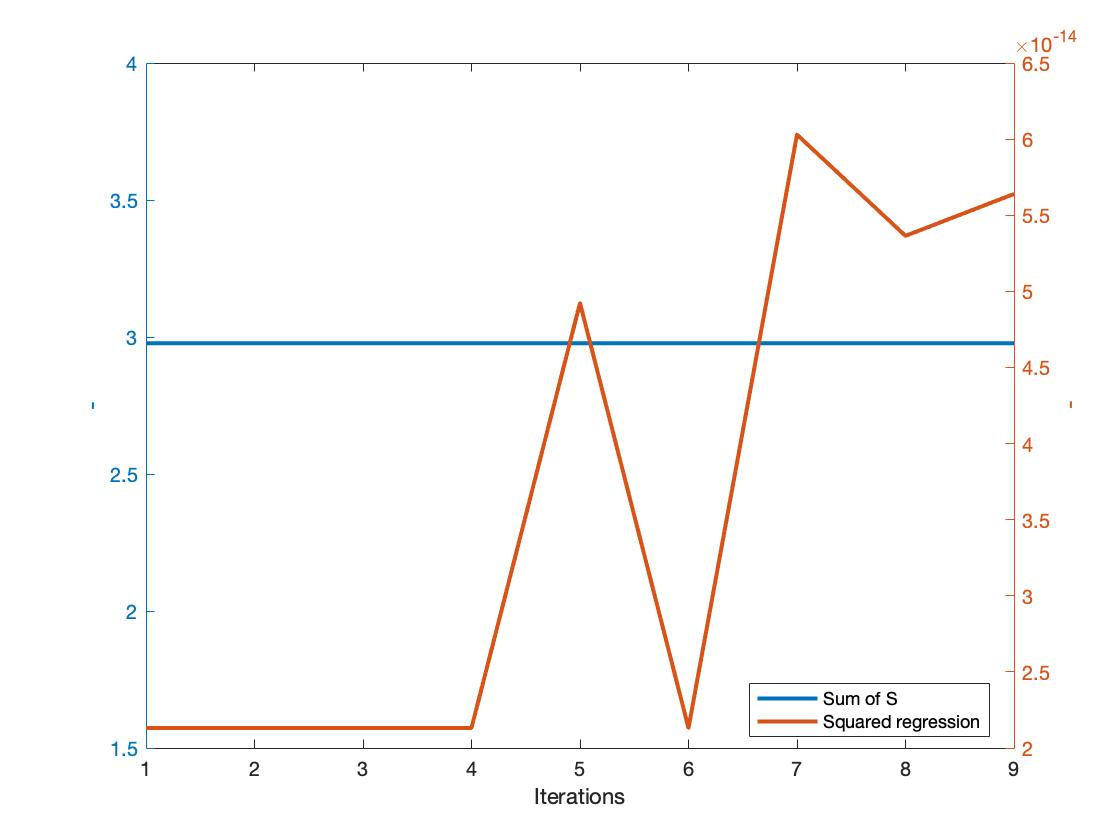
\includegraphics[width=0.45\linewidth]{../matlab/1/1reg.jpg}
	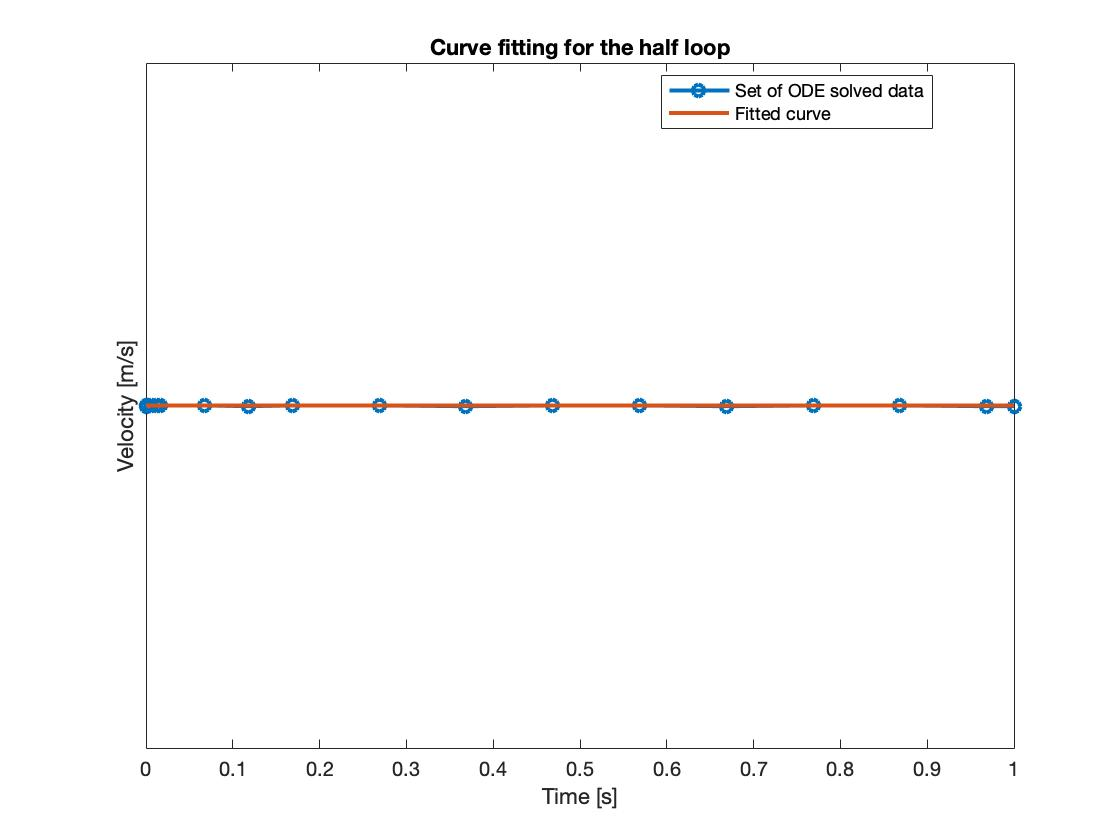
\includegraphics[width=0.45\linewidth]{../matlab/1/1fit.jpg}
	\vspace{0.5cm}
	\captionof{figure}{Lift and drag on the cruise phase. Own elaboration.}
	\label{fig:1reg}
	\captionof{figure}{Lift and drag on the cruise phase. Own elaboration.}\vspace{0.25cm}
	\label{fig:1fit}
\end{center}

\begin{center}
	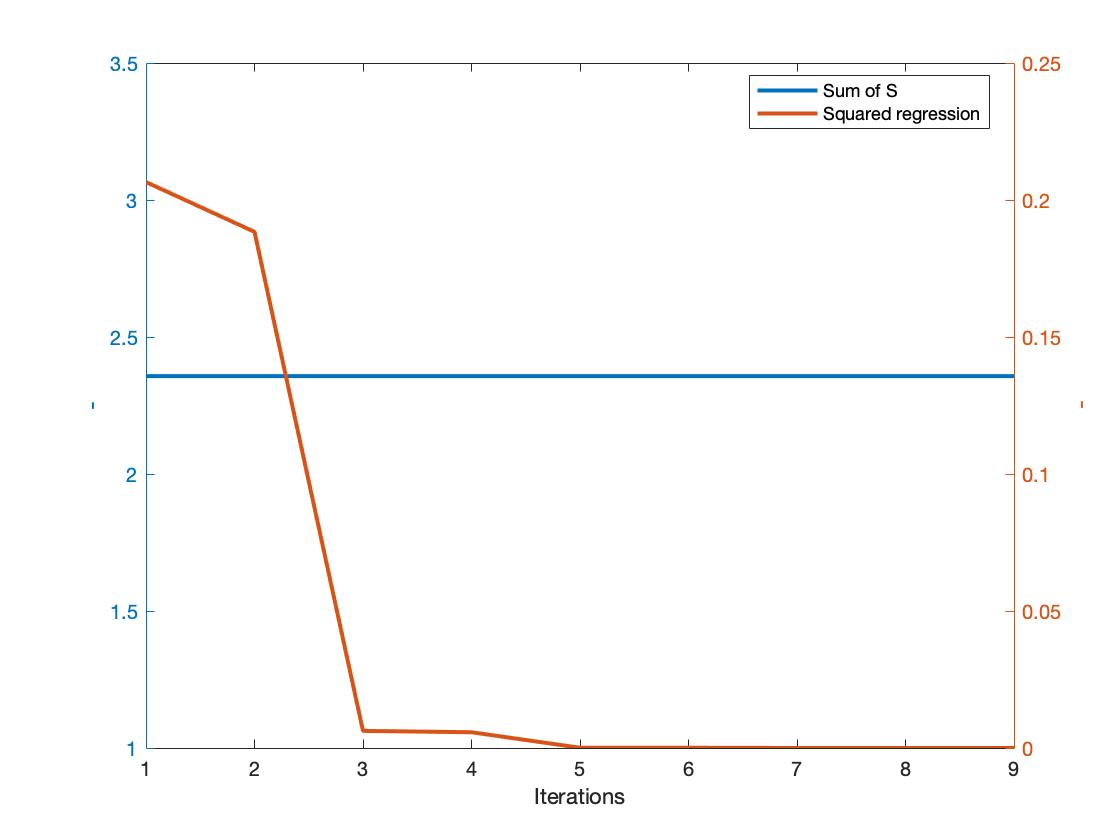
\includegraphics[width=0.45\linewidth]{../matlab/2reg.jpg}
	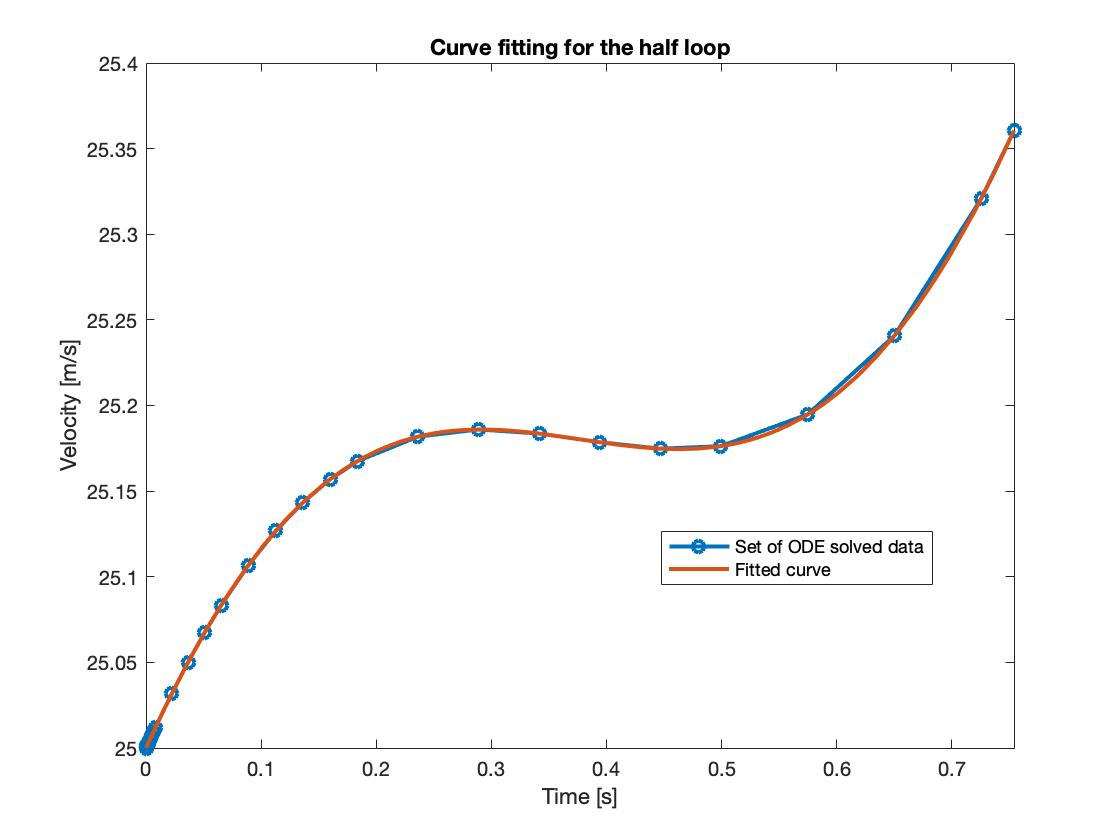
\includegraphics[width=0.45\linewidth]{../matlab/2fit.jpg}
	\vspace{0.5cm}
	\captionof{figure}{Lift and drag on the half loop. Own elaboration.}
	\label{fig:2reg}
	\captionof{figure}{Lift and drag on the half loop. Own elaboration.}\vspace{0.25cm}
	\label{fig:2fit}
\end{center}

\begin{center}
	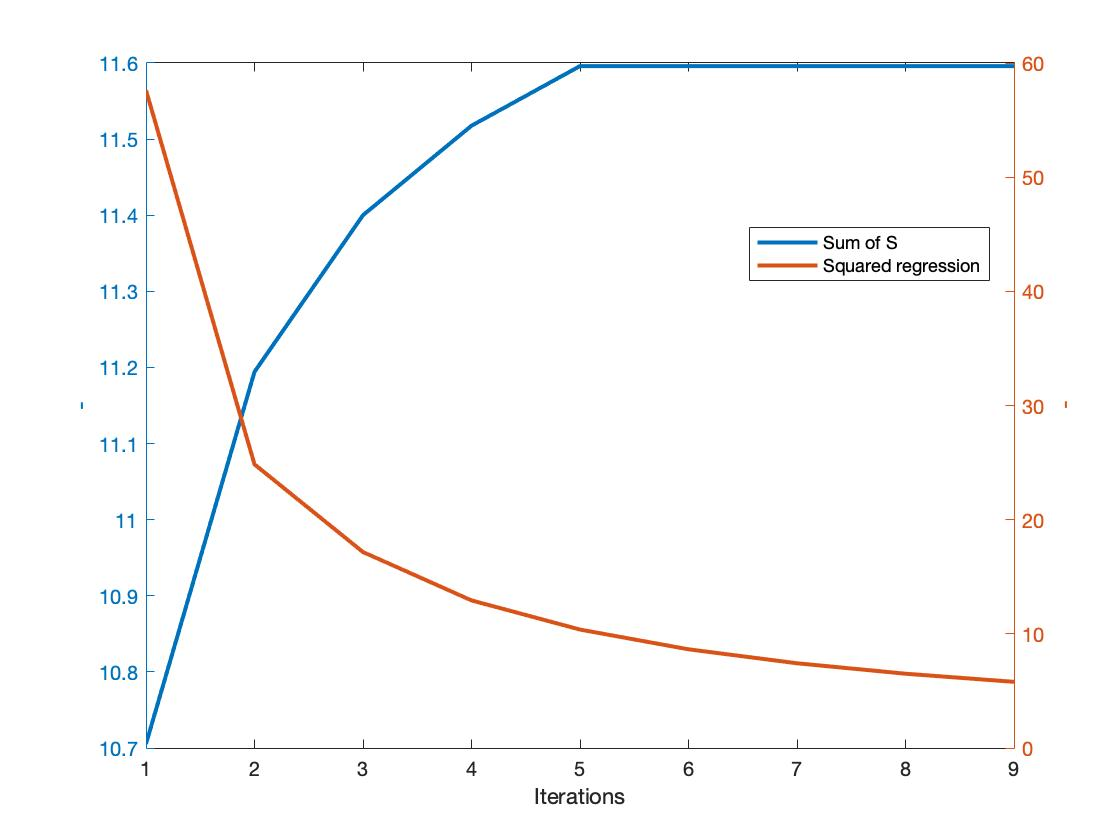
\includegraphics[width=0.45\linewidth]{../matlab/3reg.jpg}
	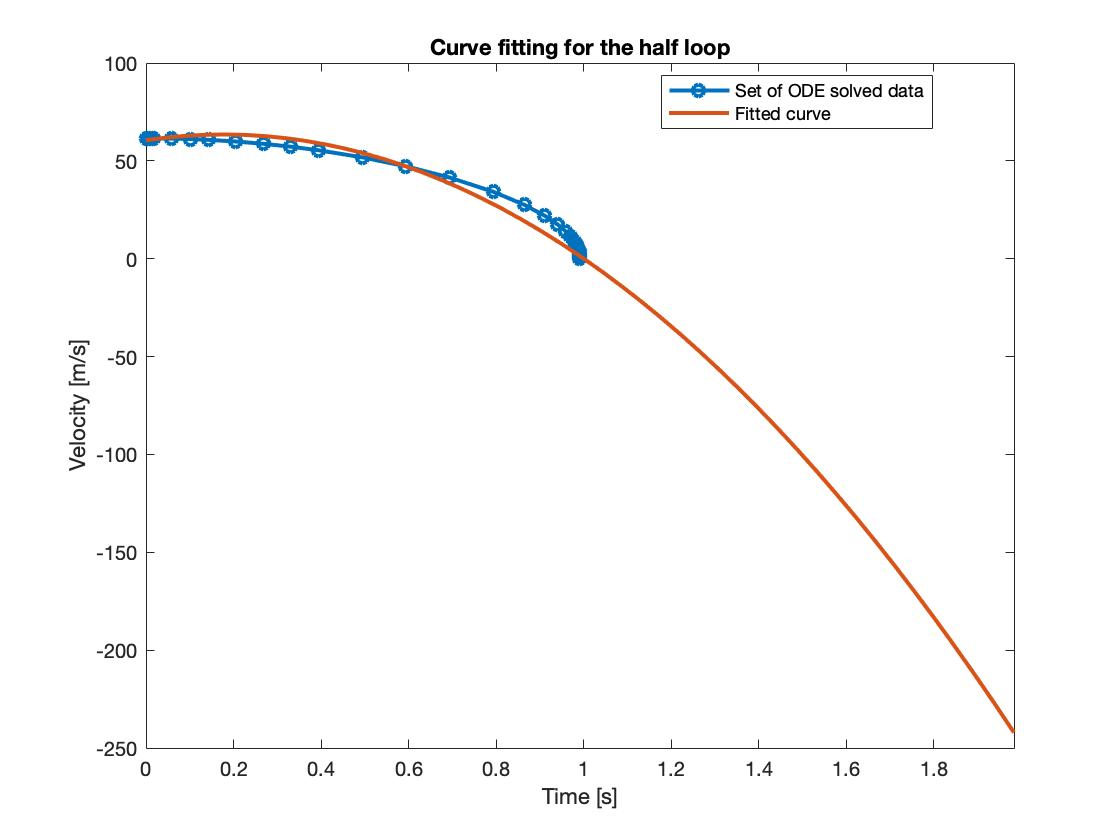
\includegraphics[width=0.45\linewidth]{../matlab/3fit.jpg}
	\vspace{0.5cm}
	\captionof{figure}{Lift and drag on the half loop. Own elaboration.}
	\label{fig:3reg}
	\captionof{figure}{Lift and drag on the half loop. Own elaboration.}\vspace{0.25cm}
	\label{fig:3fit}
\end{center}